%!TEX root = ../../../super_main.tex

\section{Help Functionality using ShowcaseView Library}
\label{sec:help_functionality_using_showcaseview_library}

It was our initial intention, as described in \secref{sec:home_screen} and seen in \figref{fig:improved_design_launch_screen} and \figref{fig:improved_design_category_selected_1}, to have some arrows with accompanying text to help guide the users with their first use of the application. We were unable to find a library which implemented such an arrow overlay, but we did however find another library called \androidinline{ShowcaseView}. \androidinline{ShowcaseView} is the name of a class and a library licensed under the Apache License, Version 2.0, originally created by Alex Curran and hosted on GitHub \parencite{showcaseview_by_alex_curran}. \androidinline{ShowcaseView} is a subclass of \androidinline{View} which, in combination with the rest of the library, can be used to showcase one or more areas of the screen. An area is showcased by putting a dark transparent overlay over the screen and then letting the showcased area, in a circle, be completely transparent along with some text as seen in \figref{fig:showcaseview_example}. Showcasing will be active through the first visit of the application and later on demand by clicking a help button. \\

\begin{figure}[!htbp]
    \centering
    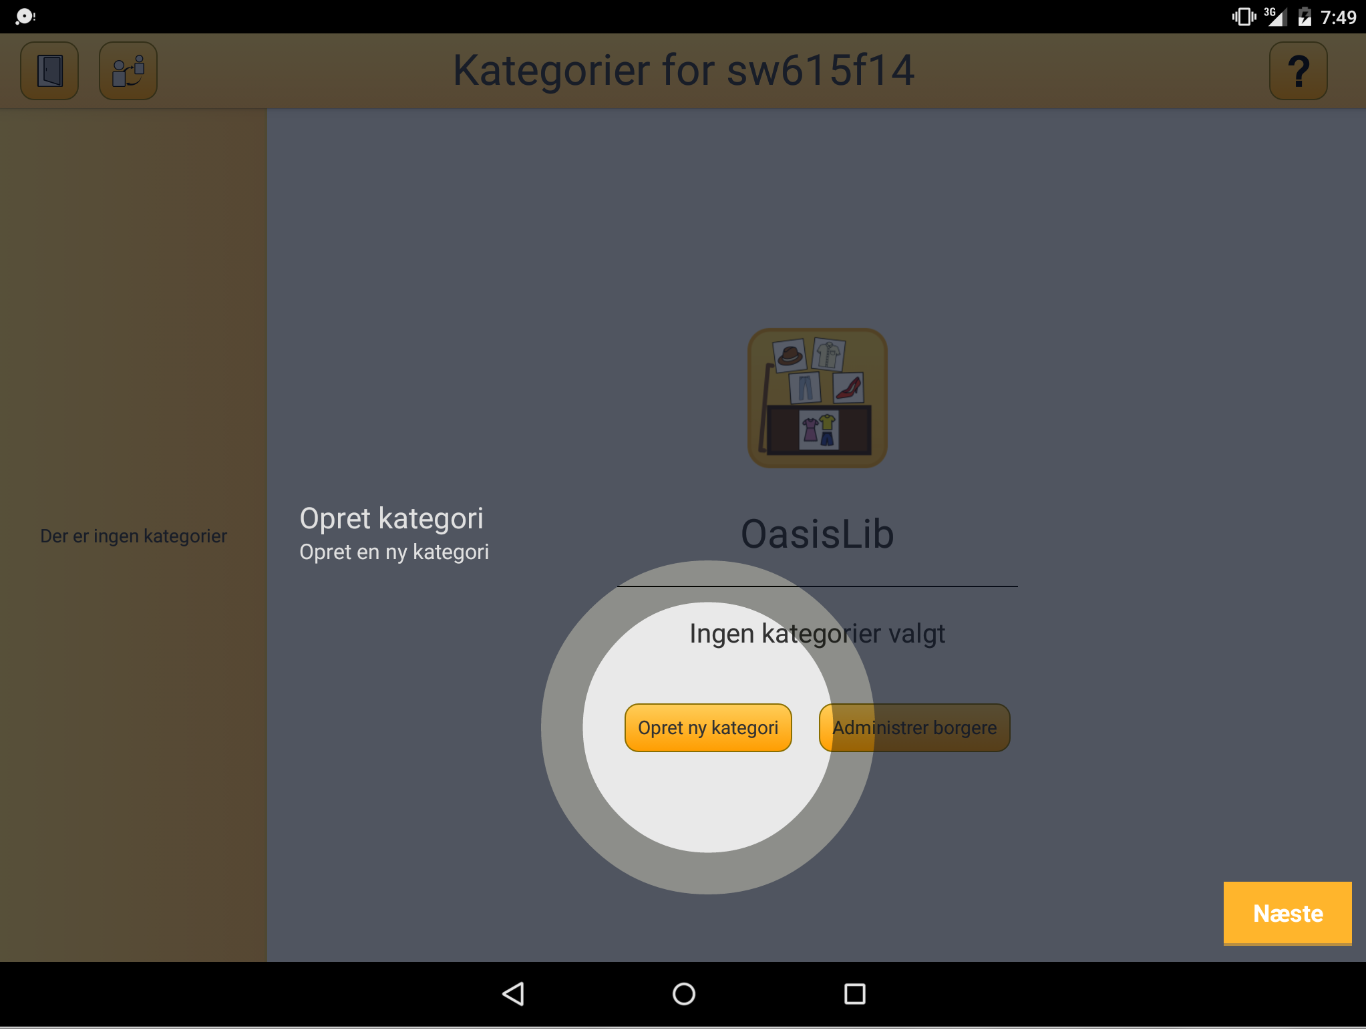
\includegraphics[width=0.75\textwidth]{sprint_three/showcaseview_example}
    \caption{Example of the \androidinline{ShowcaseView}}
    \label{fig:showcaseview_example}
\end{figure}

\subsection{Apache License}
As mentioned, this library is licensed under the Apache License 2.0 which allows for modifications and redistribution as long as certain requirements are met \parencite{apache2license}. In summary: The original copyright holder has to be credited, a full copy of the license must be distributed with the software, and changes must be stated.

\subsection{Additions to Library}

% NOTICE !!!!!! ------------> Changes here should also be made in the NOTICE file <------------
The interface \androidinline{Target} has been changed to an abstract class. And subclasses of \androidinline{Target}, i.e. classes that previously implemented the interface \androidinline{Target}, has been modified with additional constructors, methods and properties to allow them to store their radius and a \androidinline{scaleMultiplier} (This was previously hard coded). The \androidinline{ViewTarget} subclass, of \androidinline{Target}, has been further modified to calculate its own radius based on its target view.  

The \androidinline{ShowcaseView} class and supporting classes have been modified to allow manual positioning of the help text for the ShowcaseView.\\ 
The \androidinline{TextDrawer} class has been modified to fix a problem with negative widths of the drawing area.
The additions to the library code is also described in a ``NOTICE'' file which is distributed with the code in the library's root directory. 

\subsection{Supporting Code}

A new class \androidinline{ShowcaseManager} was introduced to help the transitions between different showcases. The class internally maintains a queue of objects implementing a \androidinline{Showcase} interface. A \androidinline{ShowcaseManager} instance will, when started with a call to its method \androidinline{start}, fetch the first \androidinline{Showcase} from its queue and call its \androidinline{configShowCaseView} method. This \androidinline{configShowCaseView} method is then supposed to configure the \androidinline{ShowcaseView} to match the first showcase by setting a subclass of \androidinline{Target} and more. The \androidinline{ShowcaseView} includes a next button which will, when clicked, invoke the next step by further emptying the queue and configure the next showcase.




